\begin{abstract}
\dots
\end{abstract}

\maketitle

\section{Introduction}
\label{sec:intro}
In this paper we investigate the evolution of sandpiles into states of so-called self-organized criticality (SOC) using
two different models for simulation. Furthermore we analyze the sandpiles' scaling behavior and scaling exponents.

Self-organized criticality describes a special case of the very general concept of criticality. Every system
exhibiting self-organized criticality has in common the occurrence of macroscopic scale invariant properties.
In the picture of a real sandpile this can be seen by looking at the average slope of the sandpile,
which stays constant even if the sandpile is enlarged by adding more and more sand to it.
It is notable that this is the case despite the dynamics of a pile of sand is actually governed by complicated
microscopic\footnote{Microscopic in the sense of the size of a sand grain compared to the whole pile.} interactions
of its many constituents, the sand grains.

Such self-organized criticality has been observed before in simulations of sandpiles carried out by Bak, Tang and
Wiesenfeld in the 1980s. It is indeed interesting to further analyze such a sandpile model
because it can serve as a toy model for many other similar behaving systems like landslides, rock falls, earth quakes
etc., which all follow from different physical processes, though.
In the mentioned systems signs of self-organized criticality have been observed, not only from simulations but also
from real-world data~\cite{Hergarten}.

We simulate the sandpiles using a cellular automaton algorithm analog to the approach of Bak, Tang and Wiesenfeld,
which is commonly referred to as the \enquote{BTW model}. Scaling exponents are determined and compared to the
results of a customized sandpile model.

Section~\ref{sec:theory} starts with an overview on the theory behind self-organized criticality and in particular
explains the scaling behavior governed by the scaling exponents.
In section~\ref{sec:experiment} our implementation of the sandpile cellular automata is shown as well as
the used methods for extracting the relevant parameters from the generated data.
The results are presented in section~\ref{sec:results} and discussed in section~\ref{sec:analysis}.


\section{Theory}
\label{sec:theory}

\subsection{Self-organized criticality}
\label{sec:th:SOC}
To understand the concept of self-organized criticality consider first a system that exhibits a critical state,
like the Ising model. The critical state in the Ising model corresponds to a phase transition where vanishing
magnetization evolves into spontaneous magnetization. This happens at a specific temperature, the critical temperature
$T_{\mathrm{crit}}$. To obtain a system in the critical state, the temperature has to be precisely tuned to the critical
temperature.

The criticality of the system leads to scale invariant properties. For instance clusters of the same spin direction
will form and the size distribution of these clusters follows a simple power law. A power law distribution implies
scale invariance, where scale invariance means that the dynamics of the considered system does not change if the system
is scaled by some global factor. In particular the observables' distribution functions keep the same form.

The crucial difference of this definition of criticality and the criticality observed in the case of the sandpile model
is that sandpiles will evolve into a critical state without tuning of any critical parameter.
If enough sand is deposited into a sandbox or, respectively, enough iteration steps of the computer model are performed
it reaches an equilibrium state by itself with a fixed average slope. This self-organization into a critical state
always happens, independently of the actual detailed model parameters.\footnote{Note that the slope can still depend
on these parameters.} Thus this phenomenon is called \enquote{self-organized criticality}.

\subsection{Scaling exponents}
\label{sec:th:scaling}
If there is scale invariance in a system it can be directly observed in the distribution functions
of the observables of the system as indicated above. Consider some observable $\hat{Y}$ that can be measured in the
present system. If this observable is measured many times and histogrammed one obtains a distribution according to the
corresponding probability density function $P^{Y}(y)$.
If now the system is scaled by a factor $\lambda$ it must hold
\begin{equation}\label{eq:scalingCondition}
P^{Y}(\lambda y) = f(\lambda) \times P^{Y}(y)
\end{equation}
due to the assumed scale invariance.

As scale invariance is suspected as a main property of SOC models in general, one is mainly interested in studying
these distribution functions to proof this. To do this a theoretical prediction is necessary first.
In the simplest approximation the distribution function of an observable $\hat{Y}$ in a scale invariant SOC model
is assumed to be a simple power law
\begin{equation}\label{eq:simpleScaling}
P^{Y}(y) \sim y^{-\rho}
\end{equation}
in order to fulfill Eq.~\eqref{eq:scalingCondition} as $(\lambda y)^{-\rho}\sim y^{-\rho}$.
Here $\rho$ is called the \emph{critical exponent} of the observable $\hat{Y}$.

However, in a real implementation of the sandpile model or any other SOC model one has to deal with finite system sizes
since infinitely large systems can neither be simulated nor do they exist in nature.
A finite system size limits the validity of Eq~\eqref{eq:simpleScaling} because for instance avalanche sizes on a
sandpile are naturally limited to the size of the sandpile itself. Thus a more sophisticated description of scaling
has to be used, so-called \emph{finite-size scaling} as described in \cite{SOC-book}:
\begin{equation}\label{eq:finiteSizeScaling}
P^{Y}(y) = a y^{-\rho} G^{Y}\left(\sfrac{y}{y_c(L)}\right), \quad y_c(L)=b L^K
\end{equation}
The additional scaling function $G^{Y}$ accounts for limited size corrections to the simple power law scaling
by modifying the probability density for values of $y$ in the order of the limiting \emph{characteristic scale}
$y_c(L)$. This characteristic scale where limitations eventuate can itself depend on the system size $L$,
e.g. the maximum area coverage of a two dimensional lattice is $L^2$. Thus the characteristic scale is approximately
assumed to behave as $y_c(L)=b L^K$ for any observable, where $b,K$ depend on $\hat{Y}$.
The set of the critical exponent $\rho$ together with the \enquote{observable's dimension} $K$ are
generally called finite-size scaling exponents or short scaling exponents.

One possibility to obtain the finite-size scaling exponents $\rho$ and $K$ from the measured distribution functions
is via their moments $\langle P^n\rangle$. These moments follow from Eq.~\eqref{eq:finiteSizeScaling} by integration
and as is shown in~\cite{SOC-book} in the limit of an infinitely large lattice this yields
\begin{equation}\label{eq:momentScaling}
\langle P^n\rangle \xrightarrow[L\to\infty]{} a g^{Y}(0) (bL)^{\sigma_n}, \sigma_n := K(1+n-\rho).
\end{equation}
This is as an approximation also valid for finite but large enough lattice sizes where the observable's
characteristic scale is much larger than a certain lower cutoff parameter. This lower cutoff may arise from the
detailed microscopic interactions and the discreteness of the lattice, i.e. $L \gg 1$ for a lattice divided into
discrete cells of edge length $1$ can in principle yield sufficiently good results.

Using Eq.~\eqref{eq:momentScaling} the scaling exponents could now be calculated from any measured distribution
function by doing simple linear regressions to log-log plots of different moments $\langle P^n\rangle$ against $L$.
Combining the parameters $\sigma_n$ from the regression for different $n$ provides $\rho$ and $K$.

\section{Experimental Methods}
\label{sec:experiment}

\subsection{Cellular Automata}
\label{sec:cellularAutomata}
To realize the simulation of sandpiles it is convenient to construct a cellular automaton.
A cellular automaton is an algorithm that takes values on a discrete $n$-dimensional lattice and iteratively
performs updates on all lattice sites with each updated value only depending on the old value and the values of its
nearest neighbors (and possibly random numbers). Additionally the lattice sites can be periodically perturbed,
for instance increasing the value of a randomly picked lattice site.
\dots%TODO more?

\subsection{Implementation of sandpile cellular automata}
\label{sec:sandpileImplementation}
In general a cellular automaton for a sandpile in $\mathcal{N}$ dimensions works on an $\mathcal{N}-1$ dimensional
lattice where each lattice site stands for a stack of sand grains in the left dimension. That means for example that
a real sandpile, which is three dimensional, is simulated on a two dimensional lattice reflecting the ground as $x$-$y$
plane. The entry on each site then characterizes how many grains of sand are stacked in the $z$ direction.
We will denote these lattice entries by the variable $s(\vec{r})$ in the following, with the discrete lattice sites
$\vec{r}=(x,y,\ldots)^\top$.

It can be either chosen to store the actual amount of grains in the entry $z$ or the slope with respect to the
vicinity of the stack. Both choices enable for sufficient characterization and simulation of the microscopic
dynamics of the sandpile. Choosing the slope entries, however, has the drawback that the model will then be
non-isotropic anymore, as will become clear in the following, whereas storing the actual heights can make the model
implementation a bit more complex.

Within the scope of this paper we have implemented two different cellular automata that are based on these two different
choices.

\subsubsection{The BTW model}
The first approach reflects the BTW model. The BTW model by Bak, Tang and Wiesenfeld~\cite{BakTangWiesenfeld:1987}
is the first model investigating SOC in sandpile dynamics. It uses a lattice that contains slope values and
alternatingly performs a \emph{driving} and a \emph{relaxation} of the lattice:

\textbf{Driving} generally describes the active perturbation of the lattice. For a real sandpile the perturbation
intuitively consists of adding a grain of sand to the pile at a random position. Since the BTW model deals with
slopes the addition of one grain of sand could not be achieved by just increasing $s(x,y)$ about one but the neighboring
entries would have to be changed, too. This type of driving is called \emph{conservative driving}
(see Fig.~\ref{fig:driving:cons}).
For the BTW model, however, we decided to use \emph{non-conservative driving} described by simply adding one slope
unit to the considered lattice site:
\begin{itemize}
\item $s(\vec{r}) \mapsto s(\vec{r})+1$
\end{itemize}
The non-conservative driving can be thought of as adding grains of sand to \emph{all} uphill sites with respect to
$\vec{r}$ (Fig.~\ref{fig:driving:non-cons}), which is of course unphysical but converges much faster to the
SOC state~\cite{Christensen1991}. It can still reproduce results similar to the conservative algorithm when the same,
physical, relaxation algorithm is used.

\begin{figure}[htb]
    \centering
    \begin{subfigure}{0.48\linewidth}
        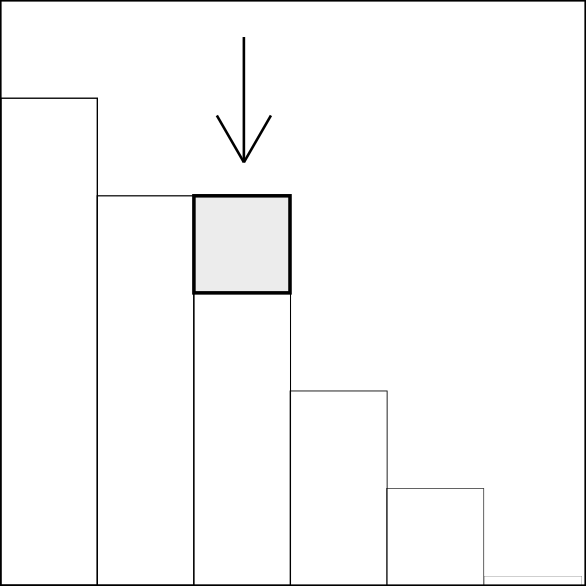
\includegraphics[width=0.85\linewidth]{drivingCons}
        \caption{Conservative driving.}
        \label{fig:driving:cons}
    \end{subfigure}
    \begin{subfigure}{0.48\linewidth}
        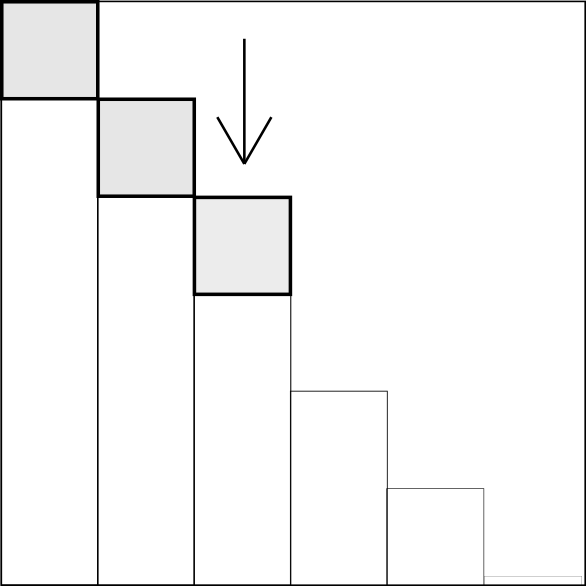
\includegraphics[width=0.85\linewidth]{drivingNonCons}
        \caption{Non-conservative driving.}
        \label{fig:driving:non-cons}
    \end{subfigure}
    \caption{Driving of a one dimensional sandpile where the columns in the sketch display
             the \emph{actual pile heights}.}
    \label{fig:driving}
\end{figure}

\textbf{Relaxation} takes place after a driving step has performed. If the sandpile becomes too steep somewhere on the
lattice, i.e. $s > s_{\mathrm{crit}}$ with the \emph{critical slope} $s_{\mathrm{crit}}$, after sand has been added
the pile gets instable. It locally collapses and thus creates avalanches of sand sliding down the pile until the slope
recovers to a non-critical value again. In the BTW model for each site with critical slope the following relaxation
algorithm is performed:
\begin{itemize}
\item $s(\vec{r}) \mapsto s(\vec{r}) - 2\times\operatorname{Dim}\left[\vec{r}\right]$
\item $s(\vec{r}\pm\vec{\mathrm{e}}_i) \mapsto s(\vec{r}\pm\vec{\mathrm{e}}_i) + 1,
\quad \forall i\in\operatorname{Dim}\left[\vec{r}\right]$
\end{itemize}
If after the relaxation any site is still critical or if any other site has become critical in the process of
relaxation the relaxation procedure is repeated until there is no critical site on the lattice anymore.
Every call of the relaxation routine counts as one unit time step.

To translate this relaxation routine to the picture of a real sandpile it calculates the local slope of the sandpile as
the sum of the local slope ($=\mathrm{stack height difference}$) in $x$-direction and the local slope in $y$-direction.
If this summed slope reaches the critical slope value $s_{\mathrm{crit}}$, for each dimension one grain of sand is
redistributed from the site to its downhill nearest neighbors This results in a consistent description of a lattice
containing slopes and the two procedures for driving and relaxation.

The fact that the slopes $s$ are only integer numbers naturally implies that they cannot contain any information about
the direction of the slope. If one takes the real sandpile picture from above into account again it becomes clear that
the slope direction is fixed to the same diagonal for every lattice point. This is a inherent feature of the BTW model
as a result of the reduction to storing slopes instead of stack heights. It creates a preferred direction for avalanches
and thus makes the model \emph{non-isotropic} such that the BTW critical state must be principally thought of as a
\enquote{diagonal hillside}.

\subsubsection{The custom model}
The second approach for the sandpile simulations uses the local height or number of sand grains as lattice entries.
Thus it can circumvent the problem of the BTW model to be non isotropic because the slopes can be directly calculated
from the heights in every direction.
The overall implementation of the custom model cellular automaton essentially follows the implementation of BTW model.
Since in the custom model the lattice entries $s(\vec{r})$ are heights instead of slopes the relaxation procedure
works differently compared to the BTW model though. \dots
The driving procedure simply consists of increasing $s(\vec{r})$ about $1$.

In the custom model it is possible to choose different boundary conditions for each edge of the lattice independently.
It can be chosen between \emph{open} and \emph{closed} boundary conditions. The closed boundaries basically model an
infinitely high wall that do not let any sand grains pass whereas the open boundaries can be thought of as the edge of
a table where any excess sand can just drop from the table. This means that sand grains can fall of the lattice at
open boundaries but accumulate at closed boundaries.
In order to make the comparison of the BTW model and the custom model possible the configuration of
$\operatorname{Dim}\left[\vec{r}\right]$ neighboring open boundaries meeting at one corner of the lattice and
respectively $\operatorname{Dim}\left[\vec{r}\right]$ neighboring closed boundaries was chosen for the simulations,
which yields a \enquote{diagonal hillside} for the custom model, too.

\subsection{Extraction of scaling exponents}
\label{sec:extractCritExp}
Since we want to study the SOC scaling behavior of sandpile avalanches we need to extract scaling exponents of
different observables. Besides the two most intuitive observables that characterize an avalanche, the \emph{area},
the \emph{time duration} and the \emph{linear size}/\emph{radius}, there is another quantity that is typically considered
in SOC studies, which is slightly misleadingly called \emph{size} of an avalanche. The size quasi describes the overall
instability released in the avalanche or also the total mass-, momentum- or energy dissipation of the avalanche.
For the automaton algorithms we precisely define all four observables as follows:
\begin{description}
\item[Size] The number of critical sites accumulated over all repititions of the relaxation procedure.
\item[Duration] The number of unit time steps from the triggering of the avalanche until it stops. The unit time step
                corresponds to one repetition of the relaxation routine.
\item[Area] The $\operatorname{Dim}\left[\vec{r}\right]-1$ dimensional volume that contains the avalanche,
            i.e. the number of lattice sites that took part in the avalanche.
\item[Linear size] The maximum (euclidean) distance between any pair of sites that took part in the avalanche.
\end{description}
The calculation of the linear size gets very computing-intensive and memory consuming for large
lattice lengths $L$ and has thus been disabled during our full simulations. In this paper we concentrate
on investigating the size, duration and area.

To each of the three considered observables needs to be assigned a set of scaling exponents $(\rho,K)$
according to Eq.\eqref{eq:finiteSizeScaling}:
\begin{description}
\item[Size] critical exponent $\tau$, avalanche dimension $D$.
\item[Duration] critical exponent $\alpha$, dynamical exponent $Z$.
\item[Area] critical exponent $\kappa$, area dimension $T$.
\end{description}

As pointed out in section~\ref{sec:th:scaling} the exponents can be determined from the corresponding measured
distributions. To obtain these distributions one full simulation run needs to be performed, which alternatingly performs
a driving and triggering of a relaxation of the lattice as described in section~\ref{sec:sandpileImplementation}.
This happens until a certain given number of drives is reached. Each relaxation between two drives corresponds to an
avalanche\footnote{Here we count no triggered avalanches as zero-size avalanches}. The desired observables are
calculated within the relaxation procedure for each avalanche and the values for all avalanches are in the end stored
by the main program. The stored data then represent samples of the underlying distribution functions.

Given a sample of one of these distributions, the distribution's first and second moment is estimated via
\begin{equation}
P^n(L) := \langle (P^{Y}(y))^n \rangle \simeq \sum_i y_i^n \Big/ \sum_i y_i^0,\quad i=1,2,
\end{equation}
where $L$ is the lattice length used in the simulation and $y_i$ the measured value of $\hat{Y}$ in the $i$-th avalanche.
According to section~\ref{sec:th:scaling} we plot $\ln\left(P^n(L)\right)$ against $\ln\left(L\right)$ using simulations
for different values of $L$ and apply a linear regression to the plot. This yields a straight line with slope $\sigma_n$,
such that $\rho, K$ follow from:
\begin{equation}
\rho = \frac{2\sigma_2 - 3\sigma_1}{\sigma_2 - \sigma_1}, \qquad\qquad K = (\sigma_2-\sigma_1)
\end{equation}

To enable for estimating uncertainties via bootstrapping, each simulation run must be applied multiple times
such that multiple samples of the distribution lead to multiple measurement values of $\ln\left(P^n(L)\right)$ for
constant $L$. We use a double bootstrap procedure in order to do a complete linear regression including the covariance
matrix of the measurement points $\langle\ln\left(P^n(L_i)\right), \ln\left(P^n(L_j)\right)\rangle$.


\section{Simulation Results}
\label{sec:results}
To achieve sufficiently good statistics also for the larger, i.e. rarer, avalanches each simulation was set up to
do $100000$ random drives and was repeated ten times for doing the bootstrap. Simulations were done for both models
in two and three dimensions for lattice lengths ranging from \SIrange{10}{100}{}.

In Figure~\ref{} \dots %TODO

\begin{figure}[htb]
    \centering
    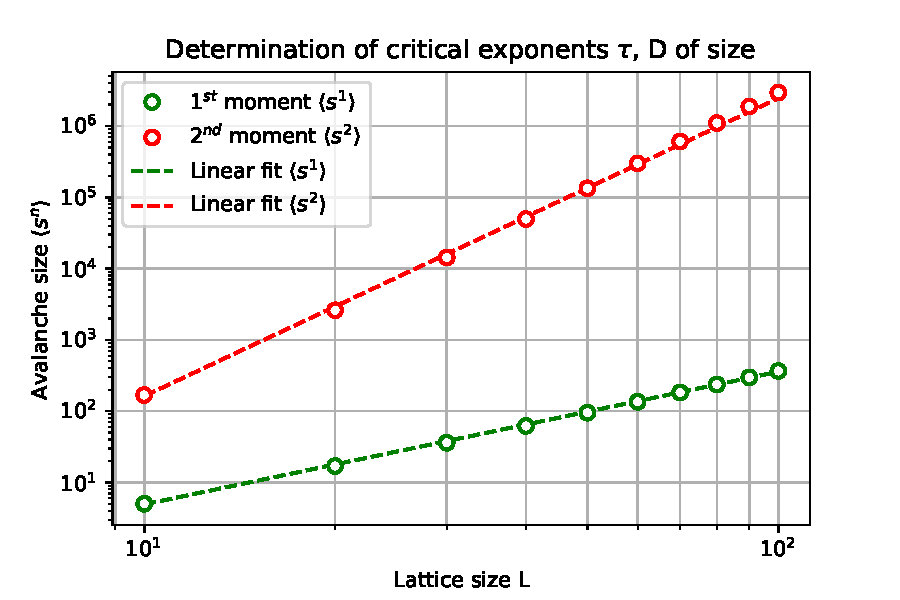
\includegraphics[width=\linewidth]{moment_analysis_size_2d_btw_fit}
    \caption{}
    \label{fig:}
\end{figure}


\begin{figure}[htb]
    \centering
    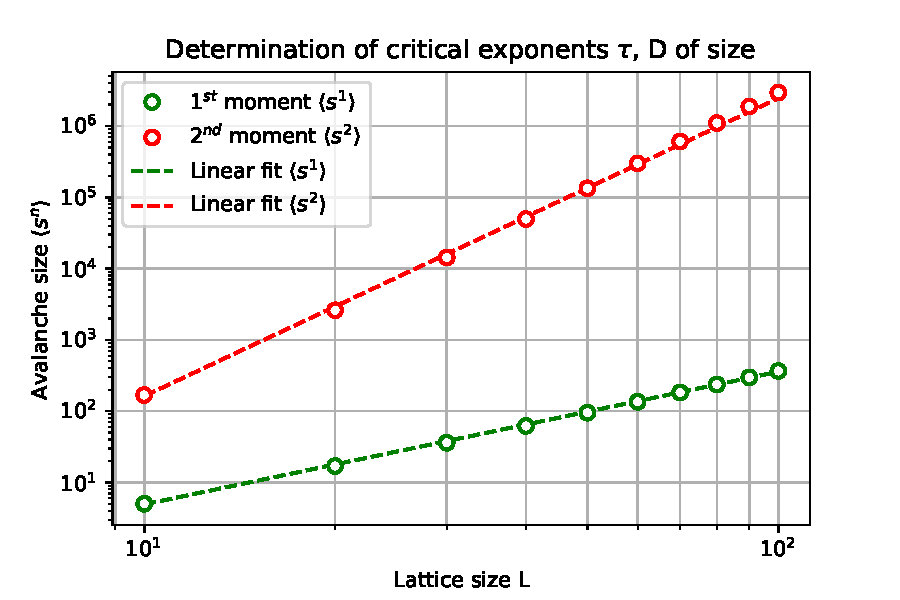
\includegraphics[width=\linewidth]{moment_analysis_size_2d_btw_fit}
    \caption{}
    \label{fig:}
\end{figure}
\begin{figure}[htb]
    \centering
    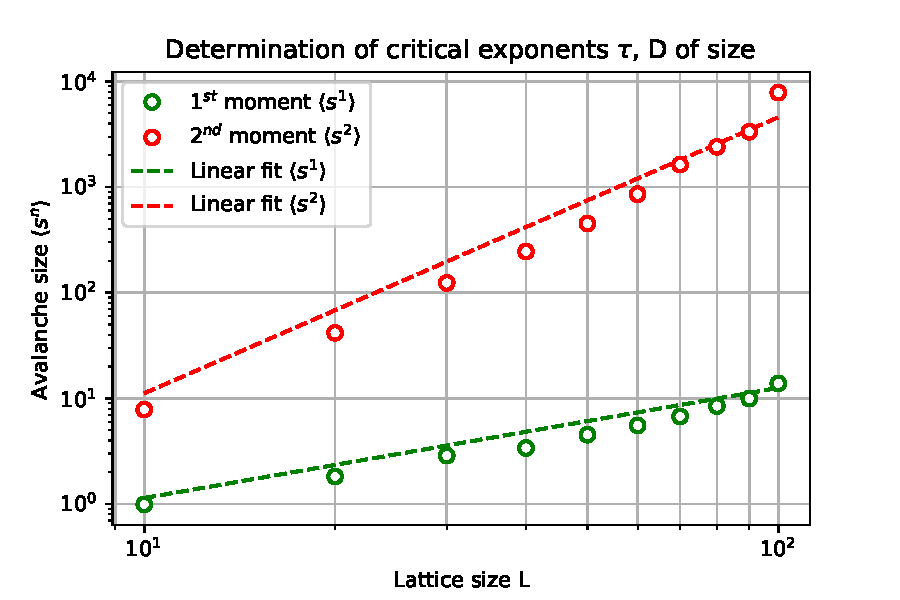
\includegraphics[width=\linewidth]{moment_analysis_size_2d_custom_crit_slope_5_fit}
    \caption{}
    \label{fig:}
\end{figure}


\section{Discussion}
\label{sec:discussion}


\section{Summary}
\label{sec:summary}


\appendix*

\section{}
\label{sec:}
\subsection{}
\dots
